\documentclass[11pt]{article}
\usepackage[margin=1in]{geometry}
\usepackage{booktabs,amsmath,amssymb,graphicx,url,array,longtable,xcolor}
\usepackage[colorlinks=true,linkcolor=blue!50!black,citecolor=blue!50!black,urlcolor=blue!50!black]{hyperref}
% AUTO-GENERATED by make_numbers.py. Do not edit.
\newcommand{\OneMismatchShared}{0/900} % H1_H3/*/O1_mismatch_rate_shared
\newcommand{\OneMismatchNaive}{0/900} % H1_H3/*/O1_mismatch_rate_naive
\newcommand{\OneMismatchKeyed}{0/900} % H1_H3/*/O1_mismatch_rate_keyed
\newcommand{\RhoTwoShared}{0.80} % H1_H3/S2/rho/shared
\newcommand{\RhoTwoSharedCI}{[0.66, 0.89]} % H1_H3/S2/rho/shared/ci
\newcommand{\RhoTwoNaive}{0.63} % H1_H3/S2/rho/naive
\newcommand{\RhoTwoNaiveCI}{[0.28, 0.82]} % H1_H3/S2/rho/naive/ci
\newcommand{\RhoTwoKeyed}{0.86} % H1_H3/S2/rho/keyed
\newcommand{\RhoTwoKeyedCI}{[0.65, 0.95]} % H1_H3/S2/rho/keyed/ci
\newcommand{\DeltaRhoTwo}{0.06} % H1_H3/S2/delta_rho_keyed_minus_shared
\newcommand{\DeltaRhoTwoCI}{[-0.16, 0.23]} % H1_H3/S2/delta_rho_keyed_minus_shared/ci
\newcommand{\DeltaRhoNaiveTwo}{0.23} % H1_H3/S2/delta_rho_keyed_minus_naive
\newcommand{\DeltaRhoNaiveTwoCI}{[-0.04, 0.58]} % H1_H3/S2/delta_rho_keyed_minus_naive/ci
\newcommand{\VRFTwo}{1.24} % H1_H3/S2/VRF_shared_over_keyed
\newcommand{\VRFTwoCI}{[0.57, 2.89]} % H1_H3/S2/VRF_shared_over_keyed/ci
\newcommand{\WidthRatioTwo}{0.88} % H1_H3/S2/H3_width_ratio_keyed_over_shared
\newcommand{\HOneVerdictTwo}{not supported} % H1_H3/S2/H1_confirmed
\newcommand{\HThreeVerdictTwo}{not confirmed} % H1_H3/S2/H3_confirmed
\newcommand{\MeanDTwoShared}{-0.040} % H1_H3/S2/H3_mean_d_shared/mean
\newcommand{\MeanDTwoSharedCI}{[-0.064, -0.017]} % H1_H3/S2/H3_mean_d_shared/ci
\newcommand{\PValTwoShared}{0.0008} % H1_H3/S2/H3_mean_d_shared/signflip_p
\newcommand{\MeanDTwoNaive}{-0.015} % H1_H3/S2/H3_mean_d_naive/mean
\newcommand{\MeanDTwoNaiveCI}{[-0.041, 0.010]} % H1_H3/S2/H3_mean_d_naive/ci
\newcommand{\PValTwoNaive}{0.2521} % H1_H3/S2/H3_mean_d_naive/signflip_p
\newcommand{\MeanDTwoKeyed}{-0.008} % H1_H3/S2/H3_mean_d_keyed/mean
\newcommand{\MeanDTwoKeyedCI}{[-0.028, 0.013]} % H1_H3/S2/H3_mean_d_keyed/ci
\newcommand{\PValTwoKeyed}{0.4535} % H1_H3/S2/H3_mean_d_keyed/signflip_p
\newcommand{\PropCDiffTwo}{0.016} % H1_H3/S2/PropC_FIFO_mean_M
\newcommand{\PropCSETwo}{0.028} % H1_H3/S2/PropC_FIFO_mean_M
\newcommand{\PropCOKTwo}{yes} % H1_H3/S2/PropC_FIFO_mean_M
\newcommand{\RhoFourShared}{0.66} % H1_H3/S4/rho/shared
\newcommand{\RhoFourSharedCI}{[0.48, 0.82]} % H1_H3/S4/rho/shared/ci
\newcommand{\RhoFourNaive}{0.75} % H1_H3/S4/rho/naive
\newcommand{\RhoFourNaiveCI}{[0.64, 0.84]} % H1_H3/S4/rho/naive/ci
\newcommand{\RhoFourKeyed}{0.69} % H1_H3/S4/rho/keyed
\newcommand{\RhoFourKeyedCI}{[0.56, 0.80]} % H1_H3/S4/rho/keyed/ci
\newcommand{\DeltaRhoFour}{0.03} % H1_H3/S4/delta_rho_keyed_minus_shared
\newcommand{\DeltaRhoFourCI}{[-0.18, 0.24]} % H1_H3/S4/delta_rho_keyed_minus_shared/ci
\newcommand{\DeltaRhoNaiveFour}{-0.05} % H1_H3/S4/delta_rho_keyed_minus_naive
\newcommand{\DeltaRhoNaiveFourCI}{[-0.22, 0.09]} % H1_H3/S4/delta_rho_keyed_minus_naive/ci
\newcommand{\VRFFour}{0.79} % H1_H3/S4/VRF_shared_over_keyed
\newcommand{\VRFFourCI}{[0.37, 1.58]} % H1_H3/S4/VRF_shared_over_keyed/ci
\newcommand{\WidthRatioFour}{1.14} % H1_H3/S4/H3_width_ratio_keyed_over_shared
\newcommand{\HOneVerdictFour}{not supported} % H1_H3/S4/H1_confirmed
\newcommand{\HThreeVerdictFour}{not confirmed} % H1_H3/S4/H3_confirmed
\newcommand{\MeanDFourShared}{-0.026} % H1_H3/S4/H3_mean_d_shared/mean
\newcommand{\MeanDFourSharedCI}{[-0.051, 0.002]} % H1_H3/S4/H3_mean_d_shared/ci
\newcommand{\PValFourShared}{0.0645} % H1_H3/S4/H3_mean_d_shared/signflip_p
\newcommand{\MeanDFourNaive}{-0.034} % H1_H3/S4/H3_mean_d_naive/mean
\newcommand{\MeanDFourNaiveCI}{[-0.058, -0.010]} % H1_H3/S4/H3_mean_d_naive/ci
\newcommand{\PValFourNaive}{0.0076} % H1_H3/S4/H3_mean_d_naive/signflip_p
\newcommand{\MeanDFourKeyed}{-0.041} % H1_H3/S4/H3_mean_d_keyed/mean
\newcommand{\MeanDFourKeyedCI}{[-0.072, -0.012]} % H1_H3/S4/H3_mean_d_keyed/ci
\newcommand{\PValFourKeyed}{0.0083} % H1_H3/S4/H3_mean_d_keyed/signflip_p
\newcommand{\PropCDiffFour}{0.007} % H1_H3/S4/PropC_FIFO_mean_M
\newcommand{\PropCSEFour}{0.027} % H1_H3/S4/PropC_FIFO_mean_M
\newcommand{\PropCOKFour}{yes} % H1_H3/S4/PropC_FIFO_mean_M
\newcommand{\RhoEightShared}{0.73} % H1_H3/S8/rho/shared
\newcommand{\RhoEightSharedCI}{[0.58, 0.85]} % H1_H3/S8/rho/shared/ci
\newcommand{\RhoEightNaive}{0.65} % H1_H3/S8/rho/naive
\newcommand{\RhoEightNaiveCI}{[0.49, 0.79]} % H1_H3/S8/rho/naive/ci
\newcommand{\RhoEightKeyed}{0.86} % H1_H3/S8/rho/keyed
\newcommand{\RhoEightKeyedCI}{[0.76, 0.92]} % H1_H3/S8/rho/keyed/ci
\newcommand{\DeltaRhoEight}{0.13} % H1_H3/S8/delta_rho_keyed_minus_shared
\newcommand{\DeltaRhoEightCI}{[-0.02, 0.30]} % H1_H3/S8/delta_rho_keyed_minus_shared/ci
\newcommand{\DeltaRhoNaiveEight}{0.21} % H1_H3/S8/delta_rho_keyed_minus_naive
\newcommand{\DeltaRhoNaiveEightCI}{[0.05, 0.37]} % H1_H3/S8/delta_rho_keyed_minus_naive/ci
\newcommand{\VRFEight}{1.37} % H1_H3/S8/VRF_shared_over_keyed
\newcommand{\VRFEightCI}{[0.75, 2.58]} % H1_H3/S8/VRF_shared_over_keyed/ci
\newcommand{\WidthRatioEight}{0.85} % H1_H3/S8/H3_width_ratio_keyed_over_shared
\newcommand{\HOneVerdictEight}{not supported} % H1_H3/S8/H1_confirmed
\newcommand{\HThreeVerdictEight}{not confirmed} % H1_H3/S8/H3_confirmed
\newcommand{\MeanDEightShared}{-0.026} % H1_H3/S8/H3_mean_d_shared/mean
\newcommand{\MeanDEightSharedCI}{[-0.058, 0.005]} % H1_H3/S8/H3_mean_d_shared/ci
\newcommand{\PValEightShared}{0.1128} % H1_H3/S8/H3_mean_d_shared/signflip_p
\newcommand{\MeanDEightNaive}{-0.035} % H1_H3/S8/H3_mean_d_naive/mean
\newcommand{\MeanDEightNaiveCI}{[-0.065, -0.004]} % H1_H3/S8/H3_mean_d_naive/ci
\newcommand{\PValEightNaive}{0.0290} % H1_H3/S8/H3_mean_d_naive/signflip_p
\newcommand{\MeanDEightKeyed}{-0.033} % H1_H3/S8/H3_mean_d_keyed/mean
\newcommand{\MeanDEightKeyedCI}{[-0.060, -0.006]} % H1_H3/S8/H3_mean_d_keyed/ci
\newcommand{\PValEightKeyed}{0.0177} % H1_H3/S8/H3_mean_d_keyed/signflip_p
\newcommand{\PropCDiffEight}{0.018} % H1_H3/S8/PropC_FIFO_mean_M
\newcommand{\PropCSEEight}{0.033} % H1_H3/S8/PropC_FIFO_mean_M
\newcommand{\PropCOKEight}{yes} % H1_H3/S8/PropC_FIFO_mean_M
\newcommand{\CostShared}{3.13} % H1_H3/S2/cost_wall_ms/shared/median_ms
\newcommand{\CostNaive}{4.18} % H1_H3/S2/cost_wall_ms/naive/median_ms
\newcommand{\CostKeyed}{7.44} % H1_H3/S2/cost_wall_ms/keyed/median_ms
\newcommand{\CostRatioKeyed}{2.38} % H1_H3/S2/cost_wall_ms keyed/shared
\newcommand{\UndelFracFIFO}{1.2\%} % H2/S2/FIFO/undelivered_fraction
\newcommand{\UndelFracFIFOCI}{[1.0\%, 1.3\%]} % H2/S2/FIFO/undelivered_fraction/ci
\newcommand{\UnderUFIFO}{-0.4\%} % H2/S2/FIFO/understatement_U
\newcommand{\UnderUFIFOCI}{[-0.5\%, -0.3\%]} % H2/S2/FIFO/understatement_U/ci
\newcommand{\UndelFracFullSASP}{1.2\%} % H2/S2/FullSASP/undelivered_fraction
\newcommand{\UndelFracFullSASPCI}{[1.0\%, 1.4\%]} % H2/S2/FullSASP/undelivered_fraction/ci
\newcommand{\UnderUFullSASP}{-0.2\%} % H2/S2/FullSASP/understatement_U
\newcommand{\UnderUFullSASPCI}{[-0.4\%, -0.1\%]} % H2/S2/FullSASP/understatement_U/ci
\newcommand{\UndelFracMeanOnly}{1.2\%} % H2/S2/MeanOnly/undelivered_fraction
\newcommand{\UndelFracMeanOnlyCI}{[1.0\%, 1.4\%]} % H2/S2/MeanOnly/undelivered_fraction/ci
\newcommand{\UnderUMeanOnly}{-0.3\%} % H2/S2/MeanOnly/understatement_U
\newcommand{\UnderUMeanOnlyCI}{[-0.4\%, -0.1\%]} % H2/S2/MeanOnly/understatement_U/ci
\newcommand{\LateDiscards}{0.00} % H2/S2/*/late_discards_per_run (max)
\newcommand{\RetryDrops}{0.00} % H2/S2/*/dropped_after_retry_per_run (max)
\newcommand{\GenPerRun}{238} % H2/S2/FIFO/generated_per_run
\newcommand{\DrainValid}{passed} % H2/drain_control/validity_check_passed
\newcommand{\DrainRows}{300} % H2/drain_control/fer0_rows
\newcommand{\DrainUndelFerOne}{0.00} % H2/drain_control/fer001_undelivered_per_run (max)
\newcommand{\RankFlip}{6\%} % H2/exploratory_ranking_flip_fraction_S2
\newcommand{\UndelThreshold}{2\%} % preregistration H2 threshold (constant)
\newcommand{\HTwoVerdict}{not material} % H2/*/all_arms_material
\newcommand{\HFourRatioFIFO}{54\%} % H4/FIFO/ratio
\newcommand{\HFourRatioFIFOCI}{[37\%, 75\%]} % H4/FIFO/ratio_ci
\newcommand{\HFourWithFIFO}{0.0049} % H4/FIFO/mean_S1_with
\newcommand{\HFourWithoutFIFO}{0.0057} % H4/FIFO/mean_S1_without
\newcommand{\HFourAbsFIFO}{0.0027} % H4/FIFO/mean_abs_diff
\newcommand{\HFourRatioFullSASP}{53\%} % H4/FullSASP/ratio
\newcommand{\HFourRatioFullSASPCI}{[38\%, 72\%]} % H4/FullSASP/ratio_ci
\newcommand{\HFourWithFullSASP}{0.0060} % H4/FullSASP/mean_S1_with
\newcommand{\HFourWithoutFullSASP}{0.0057} % H4/FullSASP/mean_S1_without
\newcommand{\HFourAbsFullSASP}{0.0031} % H4/FullSASP/mean_abs_diff
\newcommand{\HFourTrace}{0.0} % H4/FIFO/trace_control_max_abs_diff
\newcommand{\HFourVerdict}{confirmed} % H4/FIFO/violation_confirmed
\newcommand{\HFourUnits}{2.7} % H4/FIFO/mean_abs_diff x 1000 (microseconds)
\newcommand{\OFiveRate}{100\%} % H5/O5_shipped/violation_rate
\newcommand{\OFiveAttempts}{23{,}963} % H5/O5_shipped/attempts
\newcommand{\OFiveSingleRate}{0\%} % H5/O5_single/violation_rate
\newcommand{\BurstShipped}{1.25} % H5/burst_run_length/shipped
\newcommand{\BurstSingle}{1.76} % H5/burst_run_length/single
\newcommand{\BurstRel}{-29\%} % H5/burst_run_length/rel_diff
\newcommand{\BurstRelAbs}{29\%} % H5/burst_run_length/rel_diff (absolute value)
\newcommand{\BurstRelCI}{[-34\%, -24\%]} % H5/burst_run_length/ci
\newcommand{\HFiveVerdict}{confirmed} % H5/burst_run_length/material
\newcommand{\LossFreqShipped}{0.0098} % H5/loss_frequency_nobursts_shipped/freq
\newcommand{\LossFreqShippedCI}{[0.0086, 0.0111]} % H5/loss_frequency_nobursts_shipped/exact95
\newcommand{\LossFreqSingle}{0.0101} % H5/loss_frequency_nobursts_single/freq
\newcommand{\LossFreqSingleCI}{[0.0089, 0.0115]} % H5/loss_frequency_nobursts_single/exact95
\newcommand{\HSixFIFO}{0/100} % H6/FIFO
\newcommand{\HSixFullSASP}{0/100} % H6/FullSASP
\newcommand{\HSixMeanOnly}{0/100} % H6/MeanOnly
\newcommand{\HSixLeakyGlobal}{100/100} % H6/LeakyGlobal
\newcommand{\HSixLeakyLocal}{0/100} % H6/LeakyLocal
\newcommand{\HSixVerdict}{pass} % H6/pass
\newcommand{\EOneTotal}{0/500} % E1 (sum)
\newcommand{\XOneMismatch}{0} % X1 (sum of arrival mismatches)
\newcommand{\XOneRhoLow}{0.67} % X1/delta_mu_0.1/shared/rho
\newcommand{\XOneRhoHigh}{-0.06} % X1/delta_mu_2.0/shared/rho
\newcommand{\XOneRhoHighKeyed}{0.03} % X1/delta_mu_2.0/keyed/rho
\newcommand{\XTwoMShipFIFO}{0.83} % X2/shipped_FIFO/M_mean
\newcommand{\XTwoMSingleFIFO}{1.91} % X2/single_FIFO/M_mean
\newcommand{\XTwoMShipSASP}{0.57} % X2/shipped_FullSASP/M_mean
\newcommand{\XTwoMSingleSASP}{1.34} % X2/single_FullSASP/M_mean
\newcommand{\XTwoRedShip}{32\%} % X2 relative reduction shipped
\newcommand{\XTwoRedSingle}{30\%} % X2 relative reduction single
\newcommand{\XTwoUndelShip}{1.2\%} % X2/shipped_FIFO/undelivered_frac
\newcommand{\XTwoUndelSingle}{3.1\%} % X2/single_FIFO/undelivered_frac
\newcommand{\XThreeFIFO}{0/100} % X3/FIFO
\newcommand{\XThreeFullSASP}{0/100} % X3/FullSASP
\newcommand{\XThreeMeanOnly}{0/100} % X3/MeanOnly
\newcommand{\XThreeLeakyGlobal}{94/100} % X3/LeakyGlobal
\newcommand{\XThreeLeakyLocal}{20/100} % X3/LeakyLocal
\newcommand{\XFourDKeyed}{-0.014} % X4/keyed/mean_d
\newcommand{\XFourCIKeyed}{[-0.022, -0.007]} % X4/keyed/ci
\newcommand{\XFourFIFOKeyed}{0.119} % X4/keyed/mean_FIFO
\newcommand{\XFourSASPKeyed}{0.105} % X4/keyed/mean_FullSASP
\newcommand{\XFourLowerKeyed}{56\%} % X4/keyed/frac_seeds_sasp_lower
\newcommand{\XFourDShared}{-0.018} % X4/shared/mean_d
\newcommand{\XFourCIShared}{[-0.026, -0.009]} % X4/shared/ci
\newcommand{\XFourFIFOShared}{0.119} % X4/shared/mean_FIFO
\newcommand{\XFourSASPShared}{0.101} % X4/shared/mean_FullSASP
\newcommand{\XFourLowerShared}{56\%} % X4/shared/frac_seeds_sasp_lower
\newcommand{\XFourRel}{12\%} % X4 relative reduction (keyed)
\newcommand{\XFiveIdentical}{100\%} % X5/traffic_identical_fraction
\newcommand{\XFiveTriples}{270} % X5/n_triples
\newcommand{\XFiveRhoMin}{-0.32} % X5 min rho over cells
\newcommand{\XFiveRhoMax}{0.98} % X5 max rho over cells
\newcommand{\OldFIFO}{0.159} % experiments/ablation_phase6/raw_runs.csv RegimeA w50 DefaultFIFO mean weighted_cost
\newcommand{\OldSASP}{0.099} % same, FullSASP
\newcommand{\OldRel}{38\%} % same, relative reduction
\newcommand{\OldN}{30} % same, runs per arm
\newcommand{\OldD}{-0.060} % same, mean paired difference FullSASP-FIFO per seed
\newcommand{\OldDCI}{[-0.115, -0.008]} % same, seed-bootstrap 95% CI (10000, default_rng(20261017))
\newcommand{\OldRatio}{3.4} % OldD / X4 shared mean_d
\newcommand{\SBrFour}{0.7\%} % S4/FIFO/explained_fraction
\newcommand{\SBrFourCI}{[0.6\%, 0.8\%]} % S4/FIFO/explained_fraction/ci
\newcommand{\SBtauFour}{0.18} % S4/FIFO/kendall_trace_vs_shapley/mean
\newcommand{\SBtauFourCI}{[0.10, 0.27]} % S4/FIFO/kendall_trace_vs_shapley/ci
\newcommand{\SBtopFour}{39\%} % S4/FIFO/top_offender_agreement
\newcommand{\SBchanceFour}{25.0\%} % 1/4 (chance agreement)
\newcommand{\SBRFour}{1.90} % S4/FIFO/nonadditivity_R
\newcommand{\SBRFourCI}{[1.86, 1.95]} % S4/FIFO/nonadditivity_R/ci
\newcommand{\SBEFour}{1.10} % S4/FIFO/mean_E_ms
\newcommand{\SBXFour}{0.008} % S4/FIFO/mean_X_ms
\newcommand{\SBVerdictRFour}{confirmed (X does not capture externality)} % S4/FIFO/H7_verdict
\newcommand{\SBVerdictTFour}{confirmed (misranking)} % S4/FIFO/H8_verdict
\newcommand{\SBVerdictNFour}{confirmed (non-additive)} % S4/FIFO/H9_verdict
\newcommand{\SBrEight}{0.7\%} % S8/FIFO/explained_fraction
\newcommand{\SBrEightCI}{[0.6\%, 0.8\%]} % S8/FIFO/explained_fraction/ci
\newcommand{\SBtauEight}{0.16} % S8/FIFO/kendall_trace_vs_shapley/mean
\newcommand{\SBtauEightCI}{[0.10, 0.22]} % S8/FIFO/kendall_trace_vs_shapley/ci
\newcommand{\SBtopEight}{26\%} % S8/FIFO/top_offender_agreement
\newcommand{\SBchanceEight}{12.5\%} % 1/8 (chance agreement)
\newcommand{\SBREight}{2.69} % S8/FIFO/nonadditivity_R
\newcommand{\SBREightCI}{[2.60, 2.78]} % S8/FIFO/nonadditivity_R/ci
\newcommand{\SBEEight}{1.16} % S8/FIFO/mean_E_ms
\newcommand{\SBXEight}{0.008} % S8/FIFO/mean_X_ms
\newcommand{\SBVerdictREight}{confirmed (X does not capture externality)} % S8/FIFO/H7_verdict
\newcommand{\SBVerdictTEight}{confirmed (misranking)} % S8/FIFO/H8_verdict
\newcommand{\SBVerdictNEight}{confirmed (non-additive)} % S8/FIFO/H9_verdict
\newcommand{\SBVone}{0.0} % S4/FIFO/validity/V1
\newcommand{\SBVtwo}{0} % S4/FIFO/validity/V2
\newcommand{\SBVfour}{0.0} % S4/FIFO/validity/V4
\newcommand{\SBVthree}{0.10} % V3_lowload_control/explained_fraction
\newcommand{\SBVthreeStatus}{FAILED} % V3_lowload_control/passed
\newcommand{\SBLowE}{0.39} % LowLoad/FIFO/mean_E_ms
\newcommand{\SBLowX}{0.039} % LowLoad/FIFO/mean_X_ms
\newcommand{\SBNegE}{0.5\%} % max frac_negative_externality over configs
\newcommand{\SBSaspBlameA}{1.06} % S4/FullSASP/mean_blame_SH_by_flow[0]
\newcommand{\SBFifoBlameA}{1.11} % S4/FIFO/mean_blame_SH_by_flow[0]
\newcommand{\SBSaspBlameB}{0.74} % S4/FullSASP/mean_blame_SH_by_flow[1]
\newcommand{\SBFifoBlameB}{1.08} % S4/FIFO/mean_blame_SH_by_flow[1]
\newcommand{\SBSaspBlameC}{1.32} % S4/FullSASP/mean_blame_SH_by_flow[2]
\newcommand{\SBFifoBlameC}{1.10} % S4/FIFO/mean_blame_SH_by_flow[2]
\newcommand{\SBSaspBlameD}{1.27} % S4/FullSASP/mean_blame_SH_by_flow[3]
\newcommand{\SBFifoBlameD}{1.11} % S4/FIFO/mean_blame_SH_by_flow[3]
\newcommand{\SBSaspTau}{0.10} % S4/FullSASP/kendall_trace_vs_shapley/mean
\newcommand{\SBBCrossMin}{0.6\%} % 2b share_cross min (load1.0_asym0.1)
\newcommand{\SBBCrossMax}{36.6\%} % 2b share_cross max (load0.5_asym5.0)
\newcommand{\SBBCrossMed}{8.0\%} % 2b share_cross median over 12 cells
\newcommand{\SBBCrossBelowFifteen}{10/12} % 2b cells with share_cross < 15%
\newcommand{\SBBNetMin}{60\%} % 2b share_net min
\newcommand{\SBBNetMax}{99\%} % 2b share_net max
\newcommand{\SBBSelfAbs}{4.9\%} % 2b max |share_self|
\newcommand{\SBBIdentity}{1.4e-14} % 2b checks V5
\newcommand{\SBBSolo}{0.0} % 2b checks V6
\newcommand{\SBBCells}{12} % 2b number of cells
\newcommand{\SBBMaxCrossLoad}{0.5} % 2b load at max share (load0.5_asym5.0)
\newcommand{\SBBMaxCrossAsym}{5.0} % 2b asymmetry at max share (load0.5_asym5.0)
\newcommand{\SBBMinCrossLoad}{1.0} % 2b load at min share (load1.0_asym0.1)
\newcommand{\TenGapPinned}{0.1\%} % S3py H10/P256/gap/point
\newcommand{\TenGapPinnedCI}{[0.0\%, 0.4\%]} % S3py H10/P256/gap/ci
\newcommand{\TenGapShared}{99.5\%} % S3py H10/F64/gap/point
\newcommand{\TenGapSharedCI}{[99.3\%, 99.6\%]} % S3py H10/F64/gap/ci
\newcommand{\TenVSeven}{0.0026} % S3py H10/P256/V7_max_abs_E_minus_X_clean_runs
\newcommand{\TenEPinned}{0.0099} % S3py H10/P256/mean_E_ms
\newcommand{\TenESharedF}{0.935} % S3py H10/F64/mean_E_ms
\newcommand{\TwelveFlawSASPDiff}{6.09} % S3py H12/FullSASP/SH_minus_TR/mean
\newcommand{\TwelveFlawSASPCI}{[3.20, 9.16]} % S3py H12/FullSASP/SH_minus_TR/ci
\newcommand{\TwelveFlawTRvsRand}{-8.92} % S3py H12/FullSASP/TR_minus_RAND/mean
\newcommand{\ElevenMin}{4\%} % S3ns3 cells r min
\newcommand{\ElevenMax}{88\%} % S3ns3 cells r max
\newcommand{\ElevenDefined}{9} % S3ns3 n_defined
\newcommand{\ElevenMostly}{4} % S3ns3 n_mostly_explained
\newcommand{\ElevenLittle}{5} % S3ns3 n_little_explained
\newcommand{\ElevenRuns}{270} % S3ns3 n_nobulk_runs
\newcommand{\SXSixMaxStall}{3\%} % S3x X6 max frac_runs_with_stall
\newcommand{\SXSixGapLow}{0.6\%} % S3x X6 load1.0_win64 gap
\newcommand{\SXSixGapHigh}{15.6\%} % S3x X6 load1.4_win64 gap
\newcommand{\SXSixEHigh}{0.011} % S3x X6 load1.4_win64 mean_E_ms
\newcommand{\SXSixGapHighCI}{[0.0\%, 64.6\%]} % S3x X6 load1.4_win64 gap ci
\newcommand{\SXSevenFifoDiff}{-0.088} % S3x X7 FIFO unweighted SH_minus_TR mean
\newcommand{\SXSevenFifoCI}{[-0.194, 0.016]} % S3x X7 FIFO unweighted SH_minus_TR ci
\newcommand{\SXSevenSaspDiff}{0.000} % S3x X7 FullSASP unweighted SH_minus_TR mean
\newcommand{\FourCells}{19} % S4 n_cells
\newcommand{\FourDefined}{19} % S4 n_defined
\newcommand{\FourPyViol}{0/13} % S4 H13 python_violations/python_defined
\newcommand{\FourPyFloorViol}{0/13} % S4 H13 python_floor_violations
\newcommand{\FourNsViol}{0/6} % S4 H13 ns3_violations/ns3_defined
\newcommand{\FourRho}{0.93} % S4 H14 pooled rho
\newcommand{\FourRhoCI}{[0.78, 0.98]} % S4 H14 pooled ci
\newcommand{\FourRhoPy}{0.85} % S4 H14 python rho
\newcommand{\FourRhoNs}{0.60} % S4 H14 ns3 rho
\newcommand{\FourPyQMin}{0.03\%} % S4 python q min
\newcommand{\FourPyQMax}{9.4\%} % S4 python q max
\newcommand{\FourPyRMin}{0.8\%} % S4 python r min
\newcommand{\FourPyRMax}{23.0\%} % S4 python r max
\newcommand{\FourNsQMin}{8\%} % S4 ns3 q min
\newcommand{\FourNsQMax}{35\%} % S4 ns3 q max
\newcommand{\FourNsRMin}{12\%} % S4 ns3 r min
\newcommand{\FourNsRMax}{127\%} % S4 ns3 r max
\newcommand{\FourNsRAboveOne}{2} % S4 ns3 cells with r > 1
\newcommand{\FourRatioMedPy}{3.8} % S4 python median r/q
\newcommand{\FourRatioMaxPy}{26} % S4 python max r/q
\newcommand{\FourRatioMedNs}{2.4} % S4 ns3 median r/q
\newcommand{\FourNsEOverMin}{0.009} % S4 ns3 E of cells with r>1 (min)
\newcommand{\FourNsEOverMax}{0.056} % S4 ns3 E of cells with r>1 (max)
\newcommand{\FourTP}{2} % S4 H15 tp
\newcommand{\FourFP}{0} % S4 H15 fp
\newcommand{\FourFN}{2} % S4 H15 fn
\newcommand{\FourPrec}{1.00} % S4 H15 precision
\newcommand{\FourRecall}{0.50} % S4 H15 recall
\newcommand{\FourOLSSlope}{2.55} % S4 exploratory OLS slope
\newcommand{\FourOLSRsq}{0.57} % S4 exploratory OLS r2
\newcommand{\FourVTenGap}{7.1e-15} % S4 V10 identity_max_gap_all_rows
\newcommand{\FourVTenSig}{0} % S4 V10 replay_signature_violations
\newcommand{\FourVTenRows}{6800} % S4 V10 n_rows
\newcommand{\FourNsRuns}{360} % S4 V11 total ns3 runs

\newcommand{\tagC}{\textsc{conf}}
\newcommand{\tagE}{\textsc{expl}}
\newcommand{\tagP}{\textsc{pre-existing}}
\newcommand{\tagA}{\textsc{analytic}}

\title{How Far Can We Trust Paired-Seed Comparisons in Multi-Link Wi-Fi Simulation?\\
A Preregistered Oracle Audit of a Reordering Simulator}
\author{[Authors to be completed by the submitting authors]}
\date{}

\begin{document}
\maketitle

\begin{abstract}
Simulation studies of Wi-Fi~7 multi-link operation (MLO) routinely compare schedulers with seed-paired runs and report small gains.
We ask whether the implicit invariants behind such comparisons actually hold in a simulator and its evaluation protocol.
We preregistered six hypotheses (hash-committed before any confirmatory run), built exact label-free oracles with controls that must read zero where zero is guaranteed, and ran them on 100 fresh seeds at three scales.
Three preregistered hypotheses were \emph{not} supported: the shared random stream did not desynchronise arrivals across schedulers (\OneMismatchShared{} cell mismatches), keyed counterfactual noise did not tighten paired confidence intervals (width ratio \WidthRatioTwo{} at the primary scale), and survivor bias in delivered-only delay was immaterial (\UndelFracFIFO{} undelivered, below the \UndelThreshold{} threshold).
Two were confirmed: removing a competing flow changes a flow's self-blocking by \HFourRatioFIFO{} (\HFourRatioFIFOCI{}), so the claimed attribution invariance holds only on a fixed trace; and every transmission attempt consumes two loss draws instead of one (\OFiveRate{}), which shortens loss bursts by \BurstRelAbs{} and, in an exploratory run, changes absolute weighted blocking by more than a factor of two while leaving the relative scheduler ranking intact. The causality check passed for all real schedulers, with a documented blind spot to short look-ahead.
Exploratory follow-ups show that across-seed pairing strength falls from \XOneRhoLow{} to \XOneRhoHigh{} as links become asymmetric under \emph{both} shared and keyed random streams, and spans \XFiveRhoMin{} to \XFiveRhoMax{} across ns-3 cells, so weak pairing is a property of the dynamics and not of the random-number design.
A 1000-seed estimate of the scheduler's gain in the audited scenario is \XFourDShared{} (\XFourCIShared{}), versus \OldD{} (\OldDCI{}) from the earlier 30-seed campaign.
We provide the oracle battery, the controls, and a reporting checklist.
\end{abstract}

\section{Introduction}
Evaluating a packet scheduler by simulation usually means running two policies on the same seeds and testing the paired difference.
That practice quietly relies on invariants that are rarely checked: that the arms face the same exogenous traffic, that the reported metric covers every generated packet, that the random-number consumption matches the protocol specification, and that the policy cannot see the future.
Credibility problems of this kind are well documented for network simulation in general~\cite{kurkowski2005manet}; here we test them \emph{exactly}, in one concrete system, with controls.

The system is a discrete-event model of IEEE~802.11be MLO~\cite{ieee80211be2024} in which several flows share one Block-Ack reorder buffer, so a slow link can block packets of unrelated flows.
MLO scheduling and its anomalies are an active topic~\cite{lopezraventos2022mlo,carrascosa2023understanding}.
The audited repository also contains a scheduler (SASP) whose gain over FIFO had been reported from 30 seeds, which gives the audit a consequential worked example.

\paragraph{Contributions, ranked by strength of evidence.}
\begin{enumerate}
  \item \textbf{Pairing strength is a property of the dynamics, not of the random-number design.} Preregistered tests found no arrival desynchronisation and no benefit from keyed counterfactual noise~(\tagC). Exploratory sweeps show that across-seed correlation between arms falls toward zero with link asymmetry under both designs, and that pre-existing ns-3 runs show weak or negative pairing at higher load (from \XFiveRhoMax{} down to \XFiveRhoMin{}) although offered traffic was identical in \XFiveIdentical{} of \XFiveTriples{} triples~(\tagE{}, \tagP{}). We recommend reporting this correlation next to every paired test.
  \item \textbf{Small-sample effect sizes were imprecise.} In the audited scenario the 30-seed campaign gave \OldD{} (\OldDCI{}), \OldRatio{}$\times$ the 1000-seed estimate \XFourDShared{} (\XFourCIShared{}); the intervals overlap, so this is imprecision, not an error~(\tagE{}, \tagP{}).
  \item \textbf{A specification-conformance defect with a large effect on absolute numbers.} Two loss draws per attempt~(\tagC{}); an exploratory run shows its effect on weighted blocking under bursty loss~(\tagE{}).
  \item \textbf{An attribution claim holds only at trace level.} Self-blocking is unchanged when a flow's records are deleted from a trace (control: exactly zero), but changes when the flow is removed from the system~(\tagC{}).
  \item \textbf{An oracle battery with built-in blind-spot detection.} Truncate-and-rebuild causality testing passes for all real schedulers, but a release-level comparison cannot see a local one-millisecond look-ahead (\HSixLeakyLocal{}); a decision-level comparison can partly (\XThreeLeakyLocal{}, \tagE{}).
\end{enumerate}

\paragraph{What we do not claim.} We do not claim that SASP is superior or inferior in general; that the keyed design is useful in this simulator; that any result transfers to real Wi-Fi~7 hardware; or that the simulator is wrong in other respects.
No human annotation and no model-based judge were used, and none is claimed.
The study covers one simulator in depth; the ns-3 material is a re-analysis of pre-existing runs, not new ns-3 experiments.

\section{Related work and positioning}
We searched for work that audits simulation-evaluation invariants for MLO reordering. Our search was not exhaustive; claims below are \emph{to our knowledge}.
\begin{itemize}
  \item Kurkowski et al.~\cite{kurkowski2005manet} surveyed mobile ad hoc network simulation papers and found credibility shortfalls. We share the goal but test invariants of one system with executable oracles instead of surveying papers.
  \item Glasserman and Yao~\cite{glasserman1992crn} give conditions under which common random numbers reduce variance in discrete-event comparisons. Our keyed design is an instance; our contribution is a measurement showing the benefit can be absent when scheduler-induced trajectory divergence dominates.
  \item Oberst and Sontag~\cite{oberst2019counterfactual} build counterfactual trajectories with fixed exogenous noise for reinforcement learning. We transplant the idea (per-packet noise keyed by flow, index and attempt) to a network scheduler comparison.
  \item Chen et al.~\cite{chen2018metamorphic} review metamorphic testing. Our removal-of-a-flow and truncate-and-rebuild oracles are metamorphic relations; to our knowledge they have not been applied to MLO reordering simulators.
  \item Kaplan and Meier~\cite{kaplan1958nonparametric} introduced estimation under right-censoring. We use right-censored delay for packets still in flight at the horizon.
  \item L{\'o}pez-Ravent{\'o}s and Bellalta~\cite{lopezraventos2022mlo} and Carrascosa-Zamacois et al.~\cite{carrascosa2023understanding} study MLO traffic allocation and delay anomalies. They evaluate MLO behaviour; we evaluate the evaluation.
  \item The ns-3 Wi-Fi module added MLO in version 3.38 (STR mode)~\cite{ns3wifi2024}; we reuse a patched ns-3.47 build only for pre-existing runs.
\end{itemize}
Reference entries inherited from earlier project notes that we could not verify against a source during this study were deliberately left out.

\section{System under test and invariants}
The simulator (\texttt{src/mlo\_sim}) models Poisson flows, two links with EDCA-style backoff and frame errors, a 64-entry Block-Ack window, and a receiver that releases packets in sequence-number order.
Each released packet's reordering delay $\Delta_i$ is split into self-blocking $S_i$ and cross-blocking $X_i$; the weighted mean of $X_i$ is the headline metric $M$.
Five implicit invariants were written down before running anything:
\begin{description}
  \item[I1 pairing] arms run on the same seed face the same exogenous traffic;
  \item[I2 completeness] delay metrics cover every generated packet;
  \item[I3 loss draw] each attempt consumes exactly one loss draw;
  \item[I4 attribution] a flow's self-blocking does not depend on other flows;
  \item[I5 causality] a decision at time $T$ does not depend on events after $T$.
\end{description}
Reading the code also showed that the class named \texttt{OracleScheduler} uses no future information (it picks the highest-weight queue), so it cannot serve as a causality control; we replaced it by two purpose-built leaking schedulers (Amendment~1).

\section{Method}
\paragraph{Preregistration.} Hypotheses H1--H6, measures, thresholds, seeds (7000--7099), and the single-pass stopping rule were written and hashed before any confirmatory run; two amendments were also made before any such run (Section~\ref{sec:repro}). Anything run afterwards is labelled exploratory.

\paragraph{Designs.} \textbf{D0} is the shipped simulator (one shared random stream). \textbf{D1} gives each flow its own arrival stream (the naive fix). \textbf{D2} also keys every channel draw by (seed, flow, per-flow index, attempt, purpose), so a packet sees identical noise whichever scheduler serves it. D0 reproduced the unmodified simulator field for field on 45 test runs; the harness has 88 tests, and two propositions were property-tested on 500 random scenarios (arrival coupling under D1/D2, and that right-censored delay is a pointwise lower bound on drained delay and nondecreasing in the horizon).

\paragraph{Oracles and controls.} Each oracle has a control that removes exactly one cause and a validity check that must read zero where zero is guaranteed: identical arrival signatures under D1/D2 (O1); zero undelivered packets with loss-free drained runs (H2); self-blocking recomputed from the trace without the competing flow (H4); one draw per attempt in a single-draw variant (H5); a deliberately leaking scheduler that the causality test must catch (H6).

\paragraph{Statistics.} The cluster unit is the seed. Intervals are percentile bootstraps (10{,}000 resamples, fixed generator seed); pooled packet-level quantities are recomputed within each resample. $p$-values come from a paired sign-flip randomisation test because no statistics library was available. All numbers in this paper are generated from stored result files by \texttt{make\_numbers.py}.

\section{Confirmatory results (seeds 7000--7099)}
\begin{table}[h]
\centering\small
\begin{tabular}{p{0.06\linewidth}p{0.5\linewidth}p{0.3\linewidth}}
\toprule
 & Primary measure (primary scale) & Outcome \\
\midrule
H1 & $\Delta\rho=\rho_{\rm keyed}-\rho_{\rm shared}=\DeltaRhoTwo$ \DeltaRhoTwoCI; arrival mismatches \OneMismatchShared{} & \HOneVerdictTwo{} (scales 4/8: \HOneVerdictFour{}/\HOneVerdictEight{}) \\
H2 & undelivered fraction \UndelFracFIFO{} \UndelFracFIFOCI{} (threshold \UndelThreshold) & \HTwoVerdict{} \\
H3 & paired-CI width ratio keyed/shared \WidthRatioTwo{} (scales 4/8: \WidthRatioFour{}/\WidthRatioEight) & \HThreeVerdictTwo{} \\
H4 & $|\Delta S_1|/S_1=\HFourRatioFIFO$ \HFourRatioFIFOCI{}; trace control max diff \HFourTrace{} & violation \HFourVerdict{} \\
H5 & loss draws/attempt $\neq1$ in \OFiveRate{}; burst run length \BurstShipped{} vs \BurstSingle{} (\BurstRel, \BurstRelCI) & \HFiveVerdict{} \\
H6 & violating seeds: FIFO \HSixFIFO{}, FullSASP \HSixFullSASP{}, MeanOnly \HSixMeanOnly{}; global-leak control caught \HSixLeakyGlobal{} & \HSixVerdict{} \\
\bottomrule
\end{tabular}
\caption{Preregistered outcomes (\tagC). Thresholds are those fixed before the run.}
\end{table}

\paragraph{H1: pairing.} Under the shipped design the three arms saw arrival mismatches in \OneMismatchShared{} (seed, arm pair, scale) cells (D1/D2 are identical by construction). Across-seed correlation of $M$ between FIFO and FullSASP at the primary scale was \RhoTwoShared{} (shared, \RhoTwoSharedCI), \RhoTwoNaive{} (naive) and \RhoTwoKeyed{} (keyed); the keyed-minus-shared difference was \DeltaRhoTwo{} \DeltaRhoTwoCI, below the preregistered 0.30. The variance reduction factor was \VRFTwo{} \VRFTwoCI. An unplanned explanation, offered post hoc and untested, is that every attempt consumes a fixed number of draws, so work-conserving schedulers keep the stream position aligned. An oracle positive control (two shared-stream runs with different loss rates) confirmed that O1 can detect a mismatch.

\paragraph{H2: survivor bias.} About \GenPerRun{} packets were generated per run. The undelivered fraction (\UndelFracFIFO{} for FIFO, \UndelFracFullSASP{} for FullSASP) came from packets in flight at the horizon: drained runs left \DrainUndelFerOne{} undelivered per run, silent late discards were \LateDiscards{} per run, and retry drops \RetryDrops{} per run. Right-censoring made the mean delay slightly \emph{lower} (relative change \UnderUFIFO{} for FIFO), because the censored packets are the youngest; the expected direction of the bias did not appear. The loss-free drain control passed (\DrainValid{}, \DrainRows{} runs).

\paragraph{H3: consequence for the comparison.} Using the keyed design did not narrow the paired interval (width ratio \WidthRatioTwo{} at the primary scale). The point estimate of the SASP minus FIFO difference was \MeanDTwoShared{} (\MeanDTwoSharedCI, $p=\PValTwoShared$) under D0, \MeanDTwoNaive{} ($p=\PValTwoNaive$) under D1 and \MeanDTwoKeyed{} ($p=\PValTwoKeyed$) under D2. These are three different random realisations of the same estimand (FIFO means agree within two standard errors, difference \PropCDiffTwo{} vs. standard error \PropCSETwo), so we read them as a demonstration of sampling variability at 100 seeds, not as a design effect.

\paragraph{H4: attribution.} Mean self-blocking of the low-priority flow was \HFourWithFIFO{}~ms with the competitor present and \HFourWithoutFIFO{}~ms without (mean absolute per-seed difference \HFourAbsFIFO{}~ms, about \HFourUnits{}~$\mu$s). The relative change is large but the absolute size is microseconds. The trace-level control reproduced the original values exactly, so the identity holds on a fixed trace and fails as a statement about removing a flow from the system.

\paragraph{H5: loss draws.} In \OFiveAttempts{} attempts, every one consumed two draws (single-draw variant: \OFiveSingleRate{} violations). Without bursts both variants matched the configured frame error rate (\LossFreqShipped{} \LossFreqShippedCI{} and \LossFreqSingle{} \LossFreqSingleCI{}), as the validity check required. With a two-state burst channel the mean loss-burst length was \BurstShipped{} attempts shipped vs \BurstSingle{} single-draw.

\paragraph{H6: causality.} Truncating the input at 150~ms left all released packets identical for FIFO, FullSASP and MeanOnly (0 violations each) and exposed the global leak in \HSixLeakyGlobal{} seeds. The local leak was caught in only \HSixLeakyLocal{} seeds: a release-level comparison is blind to short look-ahead.

\section{Exploratory results (fresh seeds, no preregistered thresholds)}
\begin{figure}[h]
\centering
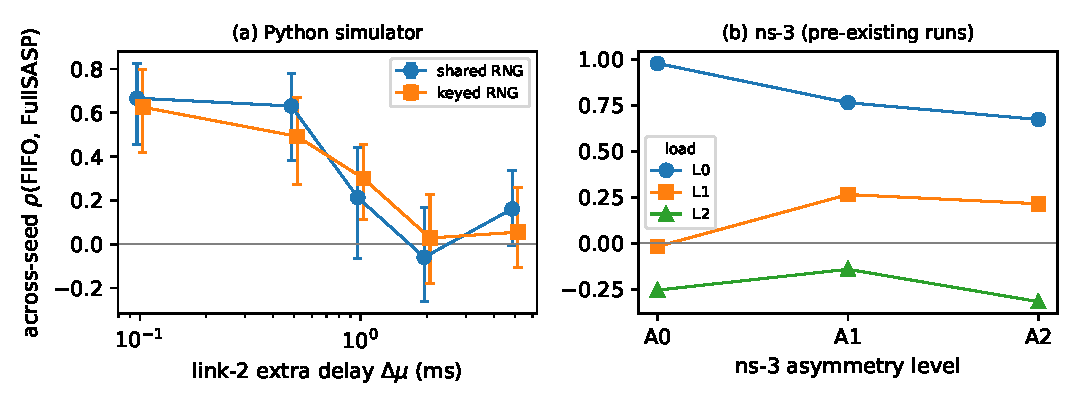
\includegraphics[width=0.95\linewidth]{fig_pairing.pdf}
\caption{Across-seed correlation between FIFO and FullSASP (\tagE{}). (a) Python simulator vs.\ link asymmetry, 100 fresh seeds per point, shared and keyed streams. (b) Pre-existing ns-3 runs (30 seeds per cell, \tagP{}).}
\end{figure}
\begin{table}[h]
\centering\small
% AUTO-GENERATED
\begin{tabular}{rcccc}
\toprule
$\Delta\mu$ (ms) & mism.\ (shared) & $\rho$ shared & $\rho$ keyed & mean $d$ keyed\\
\midrule
0.1 & 0/100 & 0.67 [0.45, 0.83] & 0.63 [0.42, 0.80] & -0.050\\
0.5 & 0/100 & 0.63 [0.38, 0.78] & 0.49 [0.27, 0.67] & -0.191\\
1.0 & 0/100 & 0.21 [-0.06, 0.44] & 0.30 [0.11, 0.46] & -0.801\\
2.0 & 0/100 & -0.06 [-0.26, 0.17] & 0.03 [-0.18, 0.23] & -3.404\\
5.0 & 0/100 & 0.16 [-0.01, 0.34] & 0.06 [-0.11, 0.26] & -16.469\\
\bottomrule
\end{tabular}

\caption{X1 (\tagE{}): asymmetry sweep, seeds 9000--9099. Arrival mismatches across arms under the shared stream totalled \XOneMismatch{} over all points and designs.}
\end{table}
\begin{table}[h]
\centering\small
% AUTO-GENERATED
\begin{tabular}{lrr}
\toprule
ns-3 cell (asym./load) & $\rho$(FIFO, FullSASP) & $n$ seeds\\
\midrule
A0 / L0 & 0.98 & 30\\
A0 / L1 & -0.02 & 30\\
A0 / L2 & -0.25 & 30\\
A1 / L0 & 0.77 & 30\\
A1 / L1 & 0.27 & 30\\
A1 / L2 & -0.14 & 30\\
A2 / L0 & 0.67 & 30\\
A2 / L1 & 0.22 & 30\\
A2 / L2 & -0.32 & 30\\
\bottomrule
\end{tabular}

\caption{X5 (\tagE{}, \tagP{}): re-analysis of the existing ns-3 campaign. Offered traffic was identical across arms in \XFiveIdentical{} of \XFiveTriples{} (cell, seed) triples.}
\end{table}
\paragraph{X1/X5: pairing strength.} Correlation fell from \XOneRhoLow{} at 0.1~ms asymmetry to \XOneRhoHigh{} at 2~ms under the shared stream and \XOneRhoHighKeyed{} under the keyed stream; arrival coupling never broke. In ns-3 the same correlation ranged from \XFiveRhoMin{} to \XFiveRhoMax{} while traffic was identical in every triple. Together these point to trajectory divergence between schedulers, not random-stream design, as the reason pairing weakens.
\paragraph{X2: effect of the double draw.} With a burst channel, weighted blocking for FIFO was \XTwoMShipFIFO{} (shipped) vs \XTwoMSingleFIFO{} (single draw), and for FullSASP \XTwoMShipSASP{} vs \XTwoMSingleSASP{}; the relative FIFO-to-FullSASP reduction was \XTwoRedShip{} vs \XTwoRedSingle{}. The undelivered fraction rose from \XTwoUndelShip{} to \XTwoUndelSingle{}. Absolute numbers depend on this specification detail; the ranking did not change.
\paragraph{X3: decision-level causality.} Comparing dispatch records instead of released packets caught the local leak in \XThreeLeakyLocal{} seeds and the global leak in \XThreeLeakyGlobal{}, with \XThreeFIFO{}, \XThreeFullSASP{}, \XThreeMeanOnly{} violations for the real schedulers.
\paragraph{X4: effect size.} Over 1000 fresh seeds the FullSASP minus FIFO difference in $M$ was \XFourDShared{} (\XFourCIShared{}) under the shipped design and \XFourDKeyed{} (\XFourCIKeyed{}) under the keyed design, about \XFourRel{} of the FIFO mean (\XFourFIFOKeyed{}); FullSASP was lower in only \XFourLowerKeyed{} of seeds. The earlier campaign (\OldN{} seeds, same scenario) had reported \OldFIFO{} vs.\ \OldSASP{} (\OldRel{} reduction).

\section{Claim-to-evidence table}
Provenance tags: \tagC{} preregistered confirmatory; \tagE{} exploratory; \tagP{} analysis of pre-existing data; \tagA{} analytic or by construction.
\begin{table}[h]
\centering\footnotesize
\begin{tabular}{p{0.32\linewidth}p{0.29\linewidth}p{0.09\linewidth}p{0.18\linewidth}}
\toprule
Claim & Evidence & Tag & Result file \\
\midrule
Shared stream does not desynchronise arrivals & \OneMismatchShared{} mismatches; \EOneTotal{} across loss rates & \tagC{}/\tagE & analysis, E1 \\
Keyed noise does not tighten paired CIs here & width ratio \WidthRatioTwo{} & \tagC & analysis \\
Pairing falls toward zero with asymmetry, both designs & \XOneRhoLow{}$\to$\XOneRhoHigh{} & \tagE & exploratory \\
ns-3 pairing varies with load & \XFiveRhoMin{} to \XFiveRhoMax{} & \tagE/\tagP & exploratory \\
Survivor bias is immaterial here & \UndelFracFIFO{} undelivered & \tagC & analysis \\
Double loss draw & \OFiveRate{} of attempts & \tagC & analysis \\
Double draw shortens bursts & \BurstRel{} (rel.\ change) \BurstRelCI & \tagC & analysis \\
Double draw changes absolute $M$ & \XTwoMShipFIFO{} vs \XTwoMSingleFIFO{} & \tagE & exploratory \\
Attribution holds only on a fixed trace & \HFourRatioFIFO{}; control \HFourTrace & \tagC & analysis \\
Real schedulers are causal (release level) & \HSixFIFO{}, \HSixFullSASP{}, \HSixMeanOnly{} & \tagC & analysis \\
Release-level test misses local look-ahead & \HSixLeakyLocal{} & \tagC & analysis \\
Gain estimate shrinks with more seeds & \OldD{} vs \XFourDShared{} & \tagE/\tagP & exploratory \\
Censoring bias direction is downward & \UnderUFIFO{} & \tagC & analysis \\
Censoring lower bound; arrival coupling (D1/D2) & 500 random scenarios & \tagA & tests/test\_props.py \\
\bottomrule
\end{tabular}
\caption{Every number resolves to a stored result file through \texttt{make\_numbers.py}.}
\end{table}

\section{Recommendations for simulation-based MLO studies}
(i) Report the across-seed correlation between arms beside every paired test, with its interval. (ii) Use enough seeds for the interval to exclude implausibly large effects; our 30-seed example did not. (iii) Add a one-draw-per-attempt check and a loss-free drained run to the simulator's test suite. (iv) State whether invariance claims hold on a fixed trace or under intervention. (v) Test causality by truncating the input, with a leaking policy as positive control, and compare decisions as well as releases.

\section{Limitations}
\begin{itemize}
  \item One simulator, two links, 300~ms runs of about \GenPerRun{} packets, and three flow-count scales. Scales are replication cells with the same thresholds, not independent evidence of a general law.
  \item Three of six preregistered hypotheses were not supported, and the arrival-coupling mechanism offered for H1 was proposed after the data and not tested by an ablation.
  \item The asymmetry sweep, double-draw effect, decision-level test, 1000-seed estimate and ns-3 comparison are exploratory; the ns-3 material re-analyses runs made before this study and no new ns-3 experiments were run, so no claim is made that the same fix or diagnosis transfers.
  \item Pilot runs on seeds 1--40 were examined before the amendment; they showed identical arrivals under the shipped design (Amendment~2 discloses this). Confirmatory seeds were untouched.
  \item The H4 effect is large in relative terms but only microseconds in absolute terms.
  \item The H6 pass is conditional on the test's power; it cannot see short look-ahead, as the control shows.
  \item The harness re-implements the event loop in a subclass; equivalence with the shipped simulator is established empirically (45 runs, field for field), not by proof.
  \item The related-work search was not exhaustive. Several reference entries inherited from earlier notes could not be verified and are omitted.
  \item $p$-values use a sign-flip randomisation test instead of a $t$-test, a deviation recorded in Amendment~2.
  \item No human annotation, no model judge and no hardware measurements were used.
\end{itemize}

\section{Conclusion}
The audited comparison's most basic invariants (same traffic across arms, complete reporting) held; two specification-level invariants did not, and the correlation that makes paired testing useful depended on system dynamics in ways that no random-number fix addressed.
The reusable outputs are the oracle battery with its controls, the reporting checklist, and the finding that effect sizes from few seeds in this setting were imprecise by a factor of about \OldRatio{}.

\section*{Reproducibility}\label{sec:repro}
Preregistration, two amendments, harness, raw results, analysis, exploratory plan and logs are in \texttt{validation/pairing/}. Commits: preregistration \texttt{4f4b8f0} (SHA-256 \texttt{abf0c16a\dots}), Amendment~1 \texttt{d7448bb} (\texttt{9c04bb72\dots}), Amendment~2 and harness \texttt{25d2ce1} (\texttt{68c09ec2\dots}), confirmatory results and exploratory plan \texttt{49437e6}. Raw-file hashes are in \texttt{results/RAW\_AND\_ANALYSIS.sha256}; decisions are logged in \texttt{decisions.md}. Rebuild with \texttt{run\_study.py}, \texttt{analyze.py}, \texttt{run\_exploratory.py}, then \texttt{paper/make\_numbers.py} and \texttt{paper/make\_fig.py}.

\bibliographystyle{plain}
\bibliography{refs}
\end{document}
